
\documentclass{article}
\usepackage[utf8]{inputenc} % 支持 UTF-8 编码
\usepackage{ctex}
\usepackage{xcolor}
\usepackage{tikz}
\usetikzlibrary{tikzmark}
\usepackage{amsmath}        % 数学公式支持
\usepackage{graphicx}       % 图片插入支持
\usepackage{geometry}       % 页面布局调整
\usepackage{lipsum}
\usepackage{tabularx}
\usepackage{xcolor} % 设置颜色
\usepackage{booktabs} % 提供美观的表格线条
\usepackage{array}    % 提供增强的列格式支持
\usepackage{multirow} % 支持多行合并单元格
\usepackage{makecell} % 支持单元格内容换行
%\usepackage[style=authoryear,backend=biber]{biblatex}
\usepackage{tikz}
\usepackage{array}
\usepackage{diagbox}
\usetikzlibrary{shapes,arrows.meta,positioning}
\usepackage[
colorlinks=true,          % 是否显示颜色而不是边框
linkcolor=blue,           % 内部链接颜色(如目录、交叉引用)
citecolor=red,            % 引用颜色
urlcolor=blue             % URL 颜色
]{hyperref}
\geometry{a4paper, margin=1in} % 设置页面边距


%\addbibresource{refs/references.bib} % 加载参考文献文件


\begin{document}
\pagenumbering{roman} % 设置页码为罗马数字
% 封面

% 封面页
\begin{titlepage}
	\centering

	% 校徽
	
\includegraphics[width=0.6\textwidth]{img/SZU_logo.png} \\
	\vspace{0.5cm} % 校徽与标题之间的间距
	
	% 标题
	\LARGE\bfseries
	综合论文题目: \\
	\vspace{0.5cm} % 标题与副标题之间的间距
	
	% 副标题
	\large\bfseries
	Chiplet技术在异质集成领域的架构设计与技术策略 \\
	\textit{(集成电路导论课程论文)} \\
	
	\vspace{2cm} % 副标题与正文信息之间的间距
	
	% 正文信息
	\begin{tabular}{l l}
		系别: & 计算机科学与技术系 \\
		专业: & 计算机科学与技术 \\
		学号: & 2025010426 \\
		姓名: & Carroll Polo \\
		指导教师: & Miller  \\
		副指导教师: & Aerith  \\
	\end{tabular}
	
	\vfill % 填充剩余空间到页面底部
	
	% 日期
	\large
	二〇二五年十月 \\
\end{titlepage}



	


%\maketitle

% 学位论文指导小组、公开评阅人和答辩委员会名单
% 本科生不需要
%\input{data/committee}

% 使用授权的说明
% 本科生开题报告不需要
%\copyrightpage
% 将签字扫描后授权文件 scan-copyright.pdf 替换原始页面
% \copyrightpage[file=scan-copyright.pdf]
%\frontmatter

% 中英文摘要和关键字
% 中文摘要
\renewcommand{\abstractname}{摘要} % 将 abstract 标题改为“摘要”
\begin{abstract}
Chiplet(芯粒)架构是一种新兴的半导体设计模式,它旨在应对摩尔定律放缓和先进工艺制造成本日益高昂的挑战。本论文系统地介绍了Chiplet架构的基本概念、特性及其在后摩尔时代集成电路设计的新范式等领域的广泛应用。以下是该篇论文的具体结构划分。

第 1 章绪论:设计目标与应用介绍介绍 Chiplet 架构的基本概念和特性(异构集成、模块化),以及 Chiplet技术的发展和应用领域(设计目标与典型应用场景);
第 2 章从“分解”的观点出发,讲述 Chiplet 划分(Die 分区)的基本理论,介绍功能分离、工艺解耦、良率优化和通信考量等概念;
第 3 章从“连接”的观点出发,讲述 2.5D/3D 封装、硅中介层和硅桥等典型微系统互连技术的一般理论和特性,给出常用的互连标准(如 UCIe)、带宽密度和相应能效参数等;
第 4 章采用“计算”与“数据”相结合的方法,讲述 Chiplet 系统的内存存储策略,其中包括高带宽内存(HBM)集成、分布式缓存一致性协议和存储层次结构等;
第 5 章介绍 Chiplet 系统中功耗与散热管理的工作原理和应用。


\end{abstract}

% 中文关键词
\noindent \textbf{关键词:} 
Chiplet (芯粒) 架构,
异构集成,
先进封装,
互连技术 / Chiplet 互连 ,
Die 分区 / 模块化设计,
高性能计算,
UCIe,
功耗与散热管理
\addcontentsline{toc}{section}{摘要} % 将摘要添加到目录中

\; 

\renewcommand{\abstractname}{Abstract} % 恢复为默认的“Abstract”


\begin{abstract}
The Chiplet architecture is an emerging semiconductor design paradigm designed to address the challenges of slowing Moore's Law and the increasing cost of advanced process manufacturing. This paper systematically introduces the basic concepts and characteristics of the chiplet architecture, as well as its broad applications in areas such as the new paradigm of integrated circuit design in the post-Moore era. The following is the detailed structure of this paper.

Chapter 1: Introduction: Design Goals and Applications introduces the basic concepts and characteristics of the chiplet architecture (heterogeneous integration and modularity), as well as the development and application areas of chiplet technology (design goals and typical application scenarios).
Chapter 2, starting from the perspective of "decomposition," discusses the basic theory of chiplet partitioning (die partitioning), introducing concepts such as functional separation, process decoupling, yield optimization, and communication considerations.
Chapter 3, starting from the perspective of "connectivity," discusses the general theory and characteristics of typical microsystem interconnect technologies such as 2.5D/3D packaging, silicon interposers, and silicon bridges, and presents commonly used interconnect standards (such as UCIe), bandwidth density, and corresponding energy efficiency parameters.
Chapter 4, taking a combined "compute" and "data" approach, describes memory storage strategies for chiplet systems, including high-bandwidth memory (HBM) integration, distributed cache coherence protocols, and storage hierarchies.
Chapter 5 introduces the working principles and applications of power consumption and thermal management in chiplet systems.


\end{abstract}

% 英文关键词
\noindent \textbf{Keywords:}
Chiplet Architecture,
Heterogeneous Integration,
Advanced Packaging,
Interconnect Technology/Chiplet Interconnect,
Die Partitioning/Modular Design,
High-Performance Computing (HPC),
UCIe,
Power and Thermal Management

\addcontentsline{toc}{section}{Abstract} % 将摘要添加到目录中

\newpage

\tableofcontents % 目录
%\addcontentsline{toc}{section}{abstract}
%\addcontentsline{toc}{section}{Abstract}

\clearpage % 强制开始新页,将目录与正文分开
% 插图和附表清单
% 本科生的插图索引和表格索引需要移至正文之后、参考文献前
% \listoffiguresandtables  % 插图和附表清单(仅限研究生)
%\listoffigures           % 插图清单
%\listoftables            % 附表清单
\pagenumbering{arabic} % 阿拉伯数字
% 符号对照表
%\input{data/denotation}


% 正文部分
%\mainmatter

\section{绪论/Introduction}

\subsection{Chiplet基本介绍}

Chiplet(芯粒)是一种模块化的处理器设计方法,将大型、复杂的芯片分解成多个功能独立的“芯粒”,这些芯粒使用标准化的通信接口(如 PCIe、HBM 或 AIB)连接在一个封装内,从而构建出高性能的系统级芯片(SoC)。这种架构的优势在于,可以利用不同的工艺节点生产不同功能的芯粒(异构集成),提高良率、降低成本,并缩短开发周期。

\begin{figure}[htbp]
	\centering
	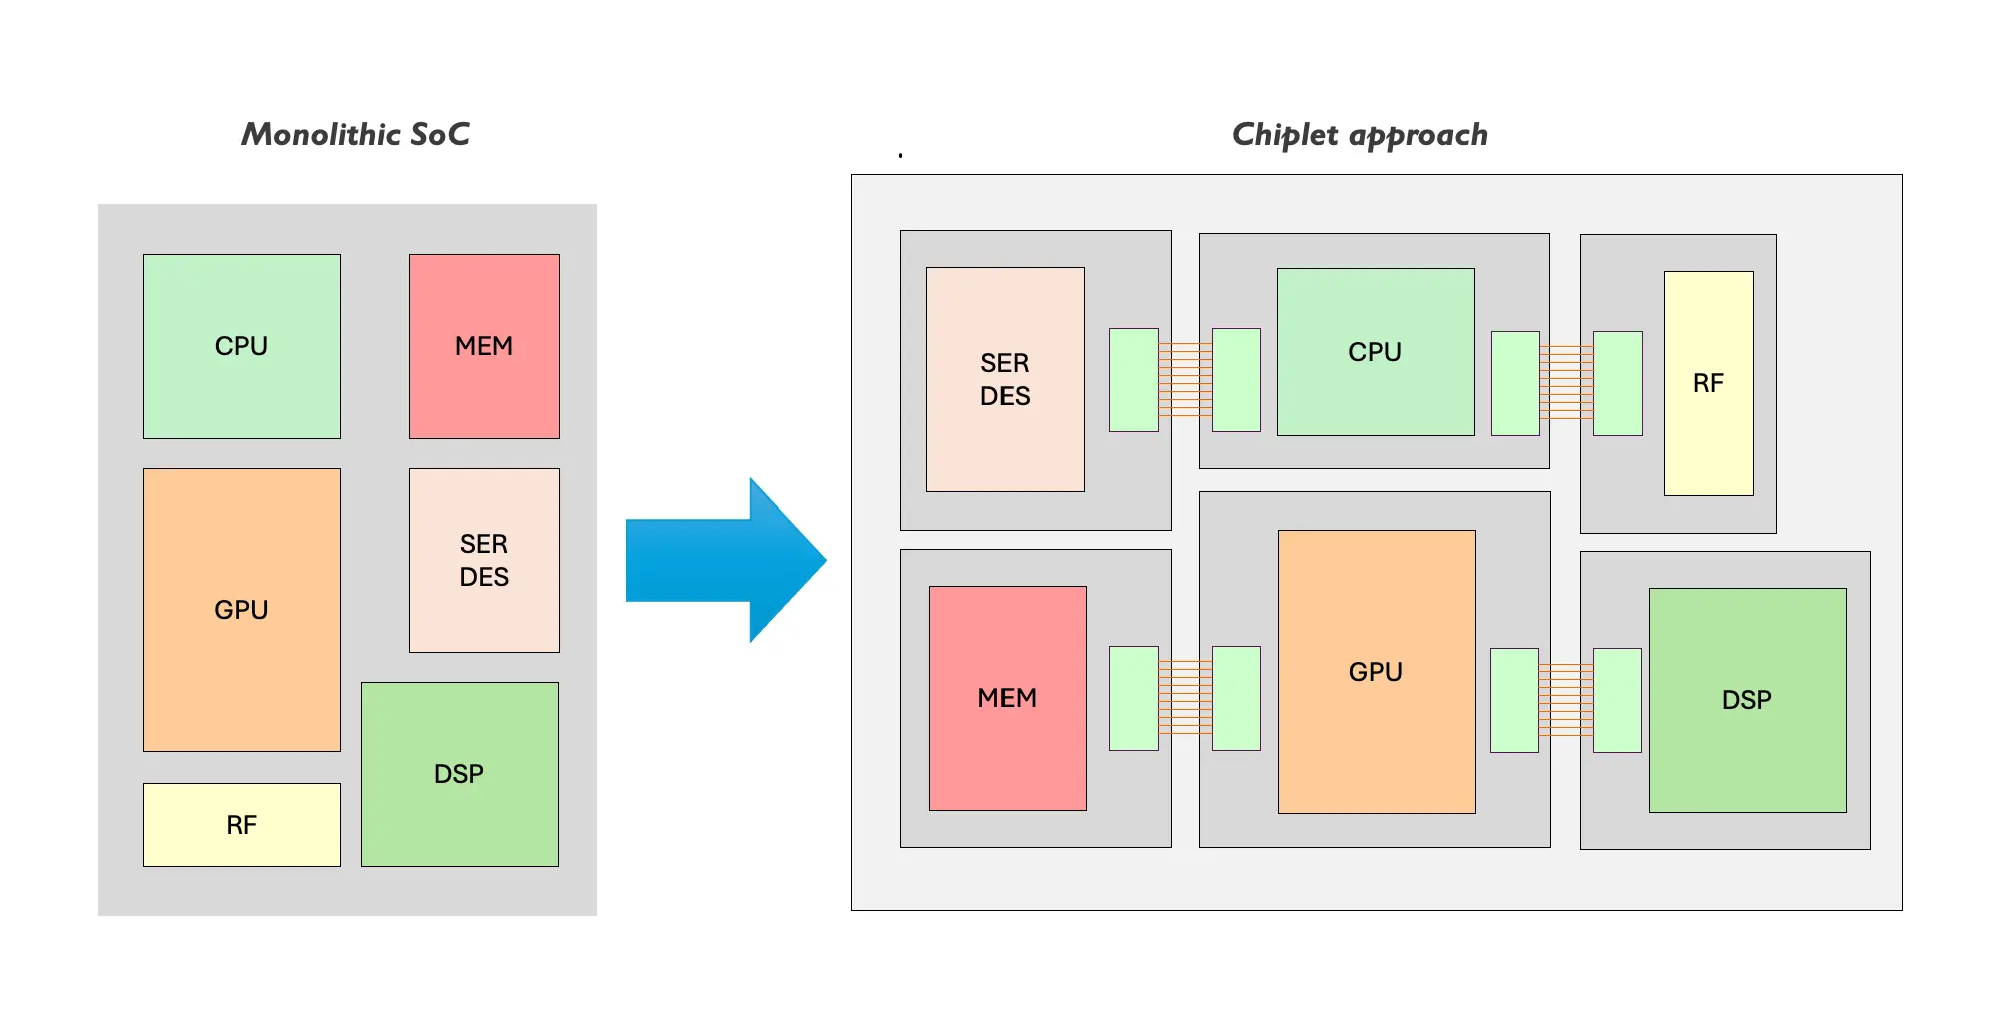
\includegraphics[width=0.8\textwidth]{img/1-1.png} % 图片文件名,不需要加扩展名
	\caption{单片集成电路片上系统与Chiplet架构系统示意图 \cite{Beyne2024Chiplet}}
	\label{fig:example}
\end{figure}

如上图所示,右侧的Chiplet架构示意图是一个微型集成电路(integrated circuit,IC),包含明确定义的功能子集。它被设计为与单个封装内插器上的其他小芯片结合在一起。一组芯粒可以在混合搭配“乐高式”堆叠组件中实现。

作为一种异构集成技术,基于芯粒的设计技术可利用先进的封装技术将不同功能的多个异构芯片集成到单个芯片中,可有效应对摩尔定律失效。随着工艺节点向前发展,成本、设计周期和复杂性急剧上升,推动业界集中芯粒领域。 芯粒可允许IC设计人员合并不同工艺节点制造的芯片,并在不同的项目中重复使用,这有助于降低设计成本,提高良率。

\subsection{采用小芯片Chiplet技术的优点}

优化性能和功耗:芯片组可以针对其特定功能和技术进行优化,从而提升系统级芯片 (SoC) 的性能和功耗。芯片组还可以更紧密地排列,从而降低互连延迟和功耗。

降低制造成本:Chiplet 可以使用不同的工艺节点和代工厂进行制造,从而降低了生产大型复杂芯片的成本和风险。Chiplet 还可以在不同的 SoC 之间重复使用,从而提高投资回报率并缩短产品上市时间。

更高的灵活性和可扩展性:芯片组可以轻松添加或移除,以调整SoC的功能和性能。芯片组的更新或替换不会影响SoC的其他部分,从而加快创新速度,并适应不断变化的市场需求。

\begin{figure}[htbp]
	\centering
	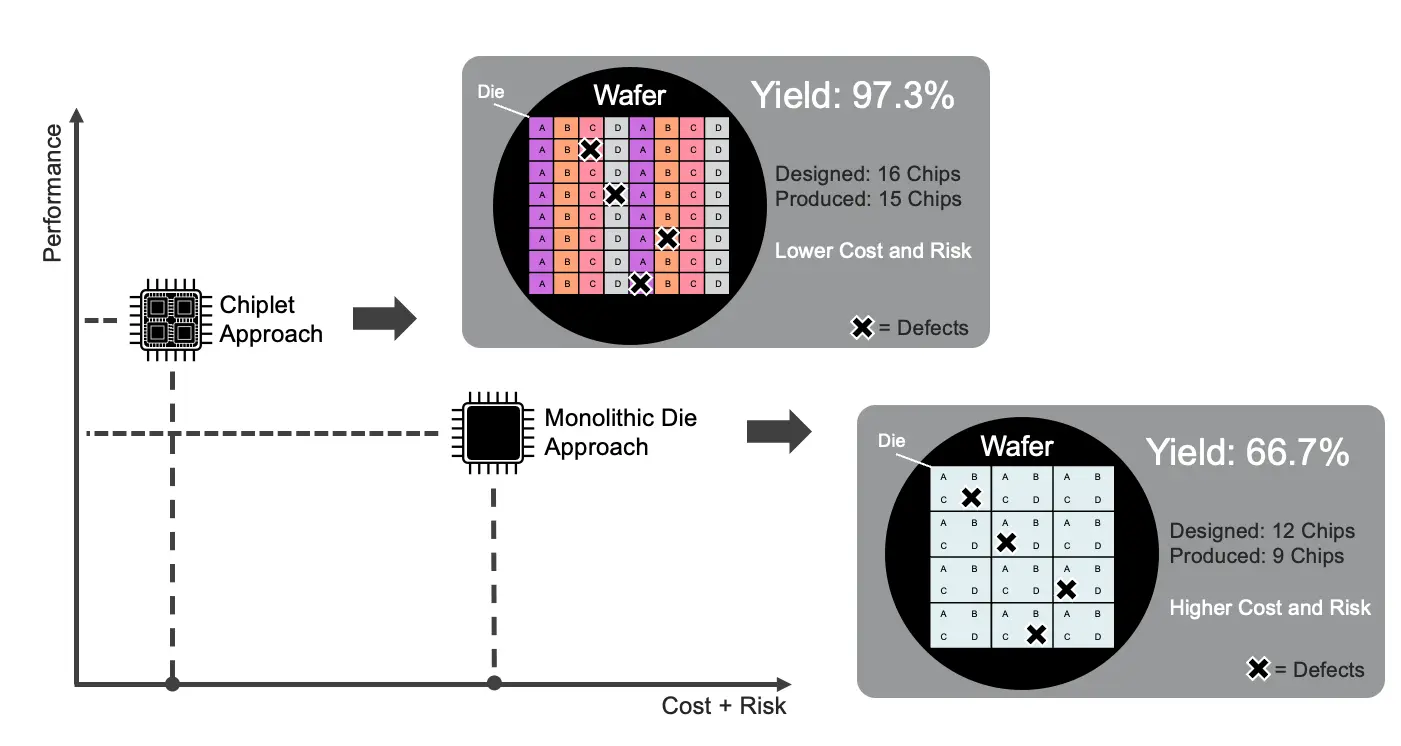
\includegraphics[width=0.8\textwidth]{img/2.png} % 图片文件名,不需要加扩展名
	\caption{小芯片与单片芯片方法的性能和成本比较 \cite{PiacentiniFilho2024Chiplet}}
	\label{fig:example}
\end{figure}

\pagebreak

\subsection{Chiplet设计的挑战}

虽然 Chiplet 的模块化方法提高了良率,但功能模块现在位于不同的芯片上,通常来自不同的供应商。设计人员无法深入探究 SoC 中每个功能 Chiplet 的内部,这增加了设计复杂性。先进的仿真和采用支持 Chiplet 工作流程的现代 EDA 解决方案成为解决这一问题的关键。

Chiplet 设计的另一个主要挑战是 Chiplet 之间的通信,即芯片间 (D2D) 通信。稳健且标准化的 D2D 通信对于确保 Chiplet 设计的可靠性和互操作性至关重要。UCIe 是一个正在兴起的开放标准,旨在标准化 D2D 通信并提高 Chiplet 设计的可靠性和互操作性。
\section{Die分区(Chiplet划分)}

首先是名词解析,“Die”(中文常译为“晶粒”或“裸芯”)是半导体制造中的一个核心术语,指从硅晶圆(Wafer)上切割下来的、一个独立的、尚未封装的微型集成电路芯片。

下面将介绍Die 在芯片制造流程中的位置以及 Die与Chiplet分区关联。

\subsection{Die 在芯片制造流程中的位置}

首先是前道工艺(Front-End-of-Line, FEOL):
在一个大的圆形硅晶圆上,通过光刻、刻蚀、薄膜沉积等数百道工序,同时制造数百到数万个完全相同的电路单元。此时,这些电路单元仍然连接在完整的晶圆上。

其次是测试与分割:通过探针(Probe)接触晶圆上的测试焊盘,对每一个电路单元(即未来的 Die)进行电气功能测试。不合格的 Die 会被标记(如点墨或记录位置)。
使用高精度金刚石锯或激光,将完成测试的晶圆切割成一个个独立的、功能完整的、合格的矩形小块。这些被切割下来的小块就是 Die(芯片裸片)。

封装测试在后道工艺(Back-End-of-Line, BEOL):
芯片键合(Die Bonding)将切割好的 Die 放置并固定(通常用粘合剂)在封装基板或引脚框架上。引线键合(Wire Bonding)用极细的金线或铜线将 Die 上的焊盘连接到封装基板或引脚框架的外部引脚上,以便 Die 能与外部电路通信。塑封(Molding)
用塑封材料(如环氧树脂)将 Die、引线和部分基板完全包裹起来,以保护其免受物理损伤和环境影响。此时,Die 变成了我们日常所见的成品芯片(IC Chip)。成品测试
对封装好的成品芯片进行最终的功能、性能和可靠性测试。

\begin{figure}[htbp]
	\centering
	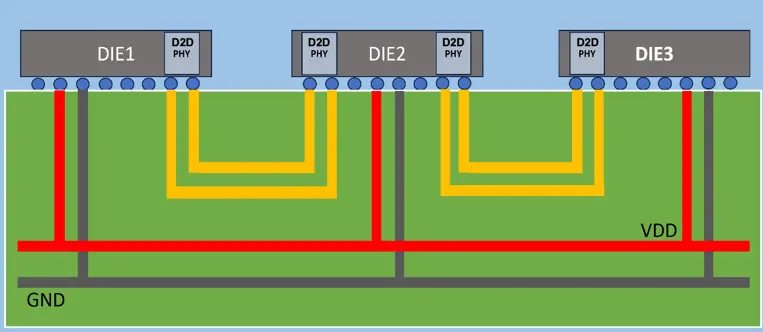
\includegraphics[width=0.6\textwidth]{img/2-1.png} % 图片文件名,不需要加扩展名
	\caption{简化的 Chiplet 标准封装视图 \cite{PiacentiniFilho2024Chiplet}}
	\label{fig:example}
\end{figure}

\subsection{Die 的应用场景}

传统的集成电路设计(如早期CPU、手机SoC)主要采用单Die芯片(Monolithic Die),将整个系统级芯片(SoC)的功能集中集成在一个晶粒上。
随着工艺发展,工业界转向了多Die系统(Multi-Die System),即在一个封装内通过先进封装技术互联多个独立制造的Die,这包括HBM内存堆叠和Chiplet架构。

在Chiplet架构中,Die分区的结果直接对应于Chiplet的划分:每个Chiplet就是一个功能独立制造的Die(芯片裸片),例如AMD CPU中的计算核心Die和I/O Die。
在Chiplet语境下,Die分区通常就是指Chiplet划分的结果——每个Chiplet就是一个独立的Die。

\begin{table}[htbp]
	\centering
	\caption{Chiplet划分与Die分区对比}
	\begin{tabular}{{c|c|c}}
		\hline
		 & Chiplet划分 & Die分区 \\
		\hline
		定义 & 功能/架构层面的模块拆分 & 物理实现层面的芯片分割 \\
		\hline
		层面 & 设计/架构层 & 物理/制造层 \\
		\hline
		目的 & 模块化、复用、异构集成 & 实现多芯片集成、提升良率 \\
		\hline
		关系 & Chiplet划分决定了Die分区的方式 & Die分区是Chiplet划分的物理实现 \\
		\hline
	\end{tabular}
\end{table}
\section{Chiplet互联技术}

芯片能否成功跟上摩尔定律,很大程度上取决于芯片在一个封装中放置的距离,以确保它们之间快速、高带宽的电连接;就像单片 SoC 中的功能一样。Chiplet 互联技术是实现多 Die 系统(Multi-Die System)的关键,它定义了封装内不同芯片裸片(Die)之间如何进行高速、低延迟、高能效的数据通信。

3D 系统集成领域正在出现两个主要的行业方向:通过公共基板(也称为中介层)并排连接芯片的 2.5D 芯片集成和 3D-SoC,其中芯片彼此堆叠。Chiplets 提供了一个模块化系统,它将来自不同供应商和技术节点的独立芯片组合在一起,而不是将所有功能设计到一个单片系统中,下面将依次介绍不同的封装方式及与之对应的互联方式。

\subsection{2D MCM封装互联}

MCM(multi chip module, 多芯片组件) 封装, 即基板平面方向
集成多个芯片或芯粒, 是比较成熟的先进封装技术, 一般是指通过引
线键合 (bonding) 或/和倒装芯片 (flip chip) 技术实现芯粒和有机
基板 (substrate, 以下简称基板) 连通, 最终芯粒之间通过基板实现
互连。因为引线键合只能在芯粒四周出连线, 互连密度低, 信号线
长, 不利于高速信号互连, 所以在chiplet中更多应用基于高密度基板
的倒装芯片MCM, 基板上的走线宽度/间距可达$9/12\mu\text{m}$, 芯粒到芯
粒的间隙可以到 $1\text{ mm}$, 保证了芯粒互连信号质量, 同时有利于缩小
封装尺寸, 控制封装成本。采用MCM封装技术的典型芯片是AMD公
司基于Zen架构的服务器和台式电脑处理器芯片, 国内寒武纪公司云
端训练芯片思元$370$也采用MCM封装形式完成 $2$ 个芯粒的互连。

\subsection{2.3D封装互联}

2.3D 封装是指在一个有机转接板上实现芯粒之间的互连, 然后再 和基板相连, 如图 4(a) 所示。它将高密度有机转接板和低密度基板 分开制造, 便于提高基板良率和降低封装成本。 2.3D 封装中有机转接 板很薄, 由于没有玻纤等增强材料, 刚度很低, 所以翘曲 (warpage) 控制是个难点。

\begin{figure}[htbp]
	\centering
	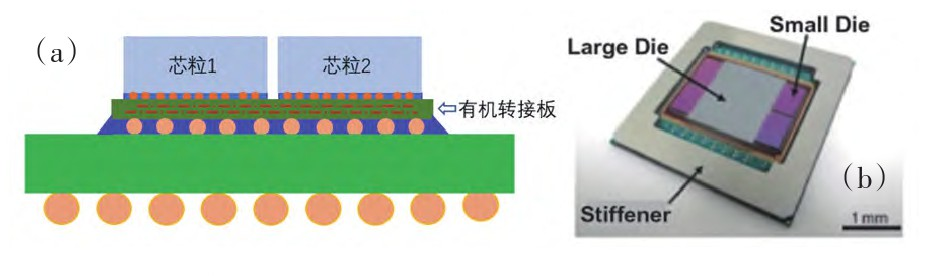
\includegraphics[width=0.6\textwidth]{img/3-2.jpg} % 图片文件名,不需要加扩展名
	\caption{$ \ 2.3\text{D}$ 封装概念图 $(\text{a})$ 及采用 $2.3\text{D}$ 封装的 $\text{Cisco}$ 公司芯片 $(\text{b})$ \cite{Miki2019Development}}
	\label{fig:example}
\end{figure}

目前有报道 Cisco 公司一款芯片已成功运用该技术, 产品线宽/间 距为 6/6μm, 集成 5 个芯粒, 如图 4(b) 
所示。国内目前已有公司 在开发双基板封装, 理念和 2.3D 封装类似, 只不过其基板互连密度没 有 2.3D 有机转接板高。

\subsection{以华为昇腾为例的Chiplet互联方式}

\begin{figure}[htbp]
	\centering
	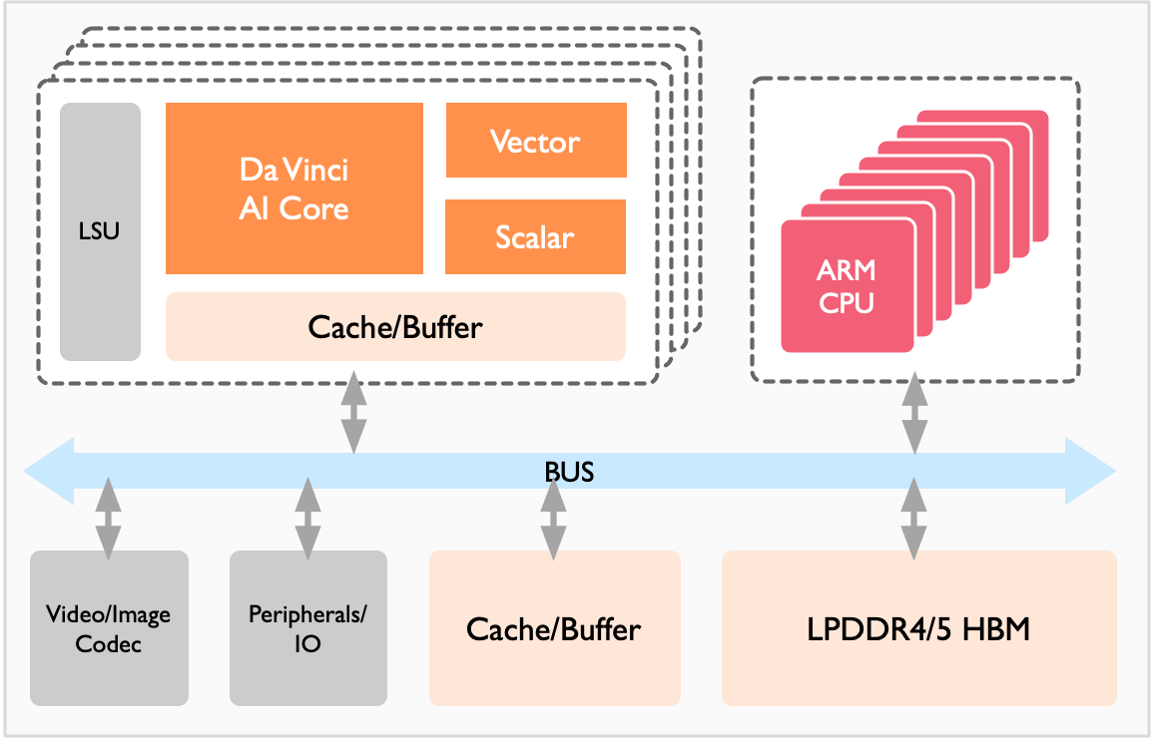
\includegraphics[width=0.6\textwidth]{img/5.png} % 图片文件名,不需要加扩展名
	\caption{基于 DaVinci AI 技术架构 \cite{CnblBlog2025}}
	\label{fig:example}
\end{figure}


昇腾 AI 处理器本质上是一个片上系统(System on Chip,SoC),主要可以应用在和图像、视频、语音、文字处理相关的应用场景。下图是早期昇腾其处理器的逻辑架构,其主要的架构组成部件包括特制的计算单元、大容量的存储单元和相应的控制单元。无论是训练还是推理的芯片以及上层的硬件型号,基于 DaVinci AI 技术架构如图5所示。

\begin{figure}[htbp]
	\centering
	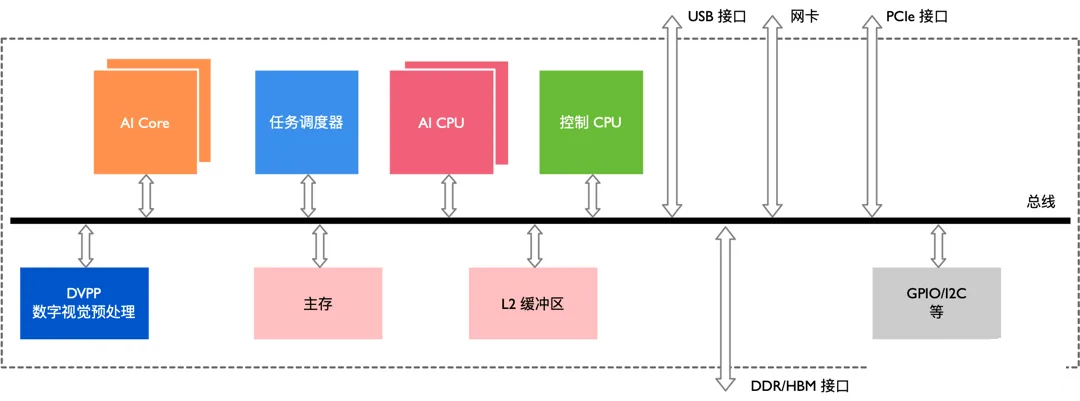
\includegraphics[width=0.8\textwidth]{img/6.png} % 图片文件名,不需要加扩展名
	\caption{ PCIe 总线接口传输总线用以实现数据互换 }
	\label{fig:example}
\end{figure}

该处理器大致可以划为:芯片系统控制 CPU(Control CPU),AI 计算引擎(包括 AI Core 和 AI CPU),多层级的片上系统缓存(Cache)或缓冲区(Buffer),数字视觉预处理模块(Digital Vision Pre-Processing,DVPP)等。芯片可以采用 LPDDR4 高速主存控制器接口,价格较低。目前主流 SoC 芯片的主存一般由 DDR(Double Data Rate)或 HBM(High Bandwidth Memory)构成,用来存放大量的数据。HBM 相对于 DDR 存储带宽较高,是行业的发展方向。其它通用的外设接口模块包括 USB、磁盘、网卡、GPIO、I2C 和电源管理接口等。

\subsection{昇腾 910的相关架构}

昇腾 910 处理器的目标场景是云端的推理和训练,其架构如图所示,包含 Davinci Core、DVPP、HBM、DDR4 等组件。

\begin{figure}[htbp]
	\centering
	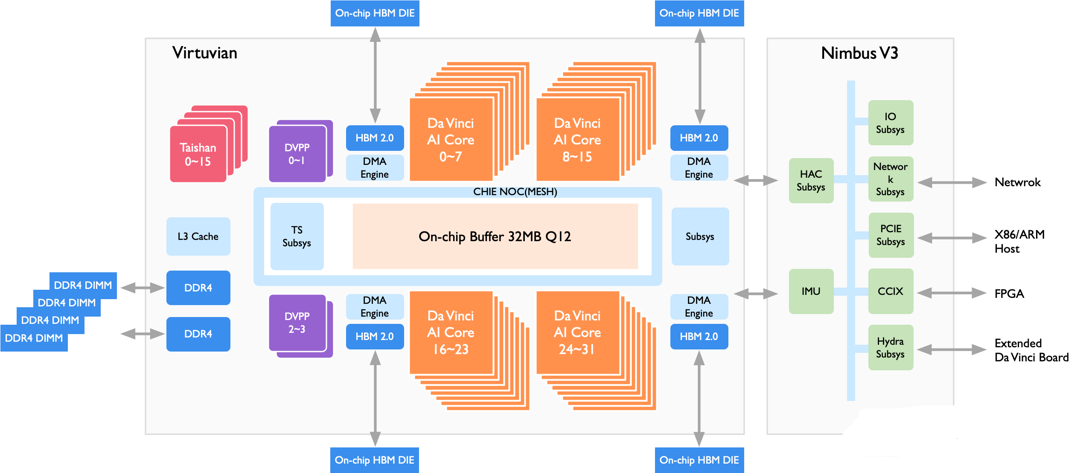
\includegraphics[width=0.8\textwidth]{img/7.png} % 图片文件名,不需要加扩展名
	\caption{昇腾 910 处理器的相关架构 }
	\label{fig:example}
\end{figure}

昇腾 910 处理器采用了芯粒(chiplet)技术,包含六个 die: 1 个计算芯粒(包含 32 个 Davinci Core、16 个 CPU Core 和 4 个 DVDP),1 个 IO 芯粒,和 4 个 HBM 芯粒(总计 1.2TB/s 带宽)。

该架构利用 AI Core 来加速通用卷积计算,总线接口从核外 L2 缓冲区或者直接从内存中读取卷积程序编译后的指令,送入指令缓存中,完成指令预取等操作,等待标量指令处理队列进行译码。如果标量指令处理队列当前无正在执行的指令,就会即刻读入指令缓存中的指令,并进行地址和参数配置,之后再由指令发射模块按照指令类型分别送入相应的指令队列进行执行。在卷积计算中首先发射的指令是数据搬运指令,该指令会被发送到存储转换队列中,再最终转发到存储转换单元中。



\section{内存存储策略}

AI应用具有数据访问和通信密集型的特点,内存访问效率与处理器运行速度的差异引发了存储墙问题,使得内存访问和通信成为性能瓶颈。

在Chiplet架构中,由于多芯粒功能划分,不会引入各个功能组件内部架构的新问题,而是需要重点考虑和解决跨芯粒所产生的问题,包括芯片互连架构和软件架构的变化。
下面以基于UCIe(Universal Chiplet Interconnect Express, 通用小芯片快连)的M.link结构为例,介绍常用的内存存储策略。

\subsection{基于UCIe的M.link的内存存储层次结构}

下图8显示了 M.Link 的层次结构,它由主结构层和次结构层、协议层、链路层和物理层组成。由于 UCIe™ 仅指定链路层和物理层支持标准和高级包的每个模块 16 和 64 个通道,因此在 M.Link 中为 D2D 接口定义了额外的层。内存控制和链路之间的结构层和协议层应支持在几纳秒的短延迟内进行数据流控制和格式转换,以降低带宽损失。M.Link 模块设计有 16 个通道,数据速率高达8GT/s,支持高达 16GBps/模块 $\texttt{\cite{Sharma2020PCIe6}}$,并且可以通过添加更多模块来增加总带宽。为了补偿时钟和数据通道之间的偏差并实现高达 10e-15 的 BER(误码率)要求,实施了使用 DLL(延迟锁定环)和 LSFR(线性反馈移位寄存器)模式的位线偏差控制和时钟训练方案。

\begin{figure}[htbp]
	\centering
	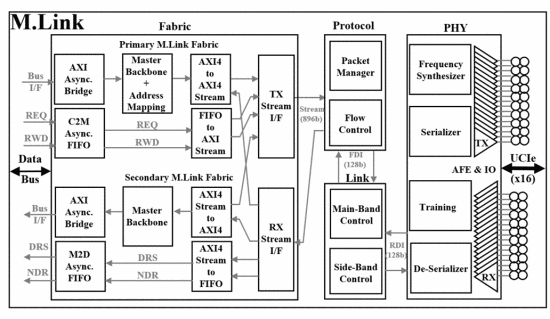
\includegraphics[width=0.6\textwidth]{img/4-1.png} % 图片文件名,不需要加扩展名
	\caption{基于UCIe™标准的M.Link框图 \cite{10848977}}
	\label{fig:example}
\end{figure}

\subsection{以M.Link为例的时钟方案}
图9中,有三种用于多芯片参考时钟的方案。使用外部晶振或内部振荡器等参考时钟源时,工作频率没有偏移。然而,第一种方案需要在电路板上增加元件,成本较高;第二种方案需要为主控制器的前向时钟提供一个I/O,功耗较大。

另一种方案在每个芯片中使用内部振荡器作为独立的参考时钟,可能会产生频率偏移。如果主控制器(快速 CLK2)的工作频率比次控制器(慢速CLK2)快,则由于吞吐量差异,次控制器的接收器无法完全恢复数据。为了保持接收器的有效带宽大于发射器的有效带宽,M.Link 使用减慢缓冲区来控制数据流,即在传输数据的中间添加一些空闲状态。尽管这会降低数据带宽,但是能极大地降低成本和提高模块组装灵活性。

\begin{figure}[htbp]
	\centering
	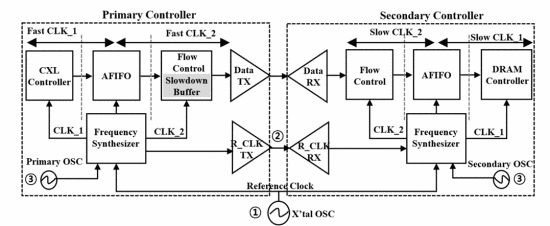
\includegraphics[width=0.6\textwidth]{img/4-2.png} % 图片文件名,不需要加扩展名
	\caption{M.Link的参考时钟方案 \cite{10848977}}
	\label{fig:example}
\end{figure}
\section{功耗与散热管理}

在平面系统级芯片(2D SoC)中,散热通常通过散热器或基板来解决。然而,在三维集成电路(3D-IC)中,为了最大程度地缩短信号传输距离,通常需要减薄基板,这会削弱基板的传热能力。此外,由于热量可能滞留在堆叠的芯片层之间,传统的散热器方案不再是最优解。



这里介绍一种EDA生产厂商的一种功耗和散热管理的方法。在EDA生产厂商模拟SoC的功耗与发热情况是,布局规划、布局、时钟和布线是模拟流程的四个主要阶段。布局规划探索发生在流程的早期阶段,设计人员将大型功能模块放置在芯片的不同区域,确定连接方式以及模块之间的布局。在此阶段,模块具有边界,将整个芯片区域划分为粗略的区域。然后,将标准单元作为定义的模块放置在每个边界内。这些是遵循代工厂设计评审手册中规则的小型库单元。然后,它们根据本地连接通过互连进行布线。总体而言,布局规划步骤包含顶层连接的抽象视图。

\begin{figure}[htbp]
	\centering
	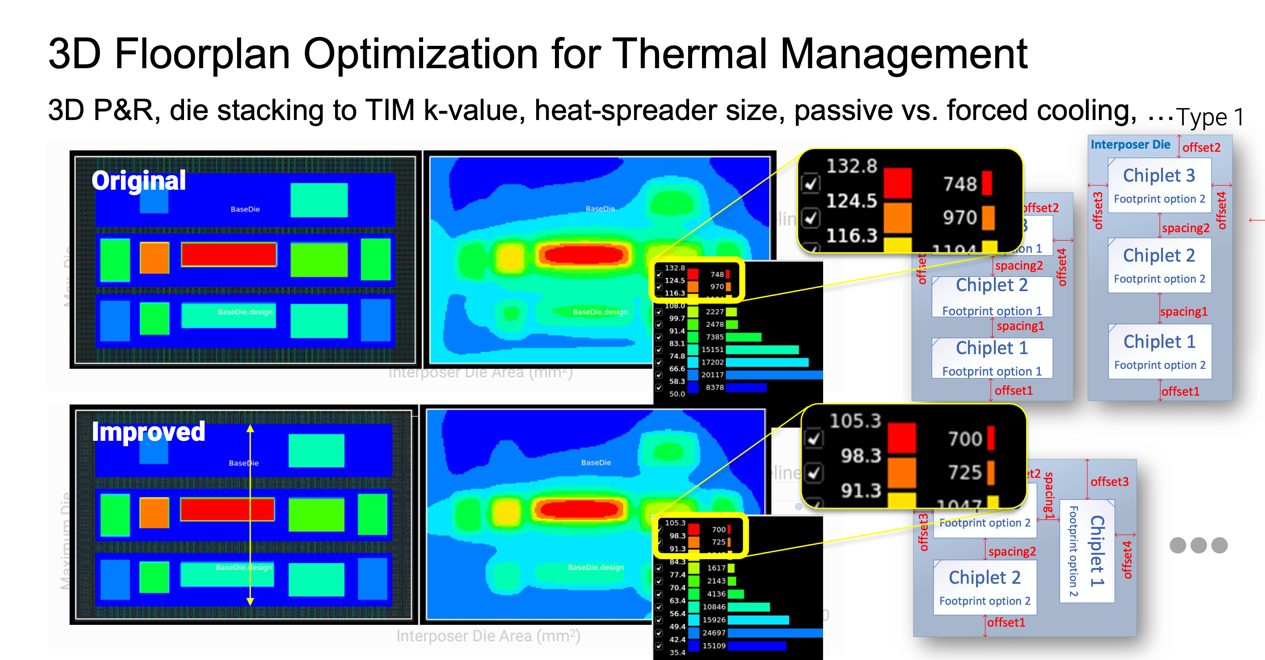
\includegraphics[width=0.8\textwidth]{img/5-1.png} % 图片文件名,不需要加扩展名
	\caption{布局规划与热管理的相互作用 \cite{Heyman2024FloorPlanning}}
	\label{fig:example}
\end{figure}

由于电压/频率调节的上下持续时间会影响性能和计算吞吐量,因此还需要进行瞬态热功率斜坡建模,并调整内部仿真温度敏感参数,例如漏电流。

集成稳压电感和用于封装设计和冷却设计的走线,系统客户还需要从芯片集设计开始的早期功率和热图,以协调组装和产品发布。因此,从寄存器传输级架构(RTL, Register-Transfer Level)之前的架构阶段到最终的流片前布局阶段 \cite{11074799},物理布局规划(包括 I/O)和一致的功率瓦特收敛也至关重要。

为了使得芯片在系统架构层面的功耗与散热管理达到一个良好的水平,需要优化芯片之间的逻辑分区。这意味着基于芯片的系统的布局布线设计流程必须考虑多芯片集成、异构技术的潜力,并管理高密度芯片间互连的复杂性。


\section{总结与展望/ConclusIon And RecommendAtIons}

随着摩尔定律逐渐逼近物理极限,传统单片式集成电路(Monolithic IC)在性能提升、成本控制和制造良率等方面面临严峻挑战。Chiplet(芯粒)架构作为一种突破性设计范式,通过将复杂系统分解为多个功能独立、可复用的小芯片模块,并利用先进封装技术实现高密度互连,有效实现了异构集成、工艺解耦与成本优化,已成为后摩尔时代集成电路发展的关键技术路径。

本文围绕Chiplet架构的核心要素,从五个维度系统性地探讨了其关键技术体系。首先,是设计目标与应用介绍介绍 Chiplet 架构的基本概念。接着在分解层面,介绍了Chiplet划分(Die分区)的基本原则,包括功能模块化、工艺节点解耦、良率优化与通信开销权衡,揭示了模块化设计如何提升设计灵活性与经济性。其次,在连接层面,深入分析了2.5D/3D封装、硅中介层(Silicon Interposer)、硅桥(Silicon Bridge)等先进互连结构,并对比了UCIe等开放互连标准的技术特性,强调了高带宽、低延迟、高能效互连对系统性能的关键影响。再次,在计算与数据协同的内存存储与传输层面,探讨了Chiplet系统中的内存架构设计,重点介绍了高带宽内存(HBM)的集成方式、分布式缓存一致性协议(如MESI、MOESI扩展)以及多层次存储体系的构建策略,以缓解“内存墙”问题。最后,在功耗与散热管理层面,阐述了Chiplet系统中局部热点管理等关键技术,以及介绍EDA厂商如何使用仿真模拟设计低功耗与散热良好的系统,用以确保系统在高性能运行下的可靠性与稳定性。





% 其他部分
%\backmatter

%\appendix
%\input{data/appendix}
\newpage
% 参考文献

\addcontentsline{toc}{section}{参考文献} % 将参考文献添加到目录中

\bibliographystyle{unsrt}
\bibliography{refs/references}



\end{document}
